
\documentclass[a4paper, 10pt, conference]{ieeeconf}      % Use this line for a4
% paper
\usepackage{hyperref}
\usepackage{graphicx}
\usepackage{amsmath}
\usepackage{float}
\usepackage[style = numeric, sorting = none]{biblatex}
\addbibresource{bibliography.bib}
\usepackage{fontspec}
\graphicspath{{./Figures/}}
\IEEEoverridecommandlockouts                              % This command is only
                                                          % needed if you want to
                                                          % use the \thanks command
\overrideIEEEmargins


\title{ 
\includegraphics[scale=.5]{logo.png}  \\
\large Innovation Ecosystem Built on the Blockchain. \\ Token Ticker - MTX \\ Updated \today
}


\author{Steve McCloskey$^{1}$, Keita Funakawa$^{2}$, Vincent Brunet$^{3}$ \\
Scott Morgan$^{4}$, Edgardo Leija$^{5}$, Adam Simon$^{6}$, Kyle Lee$^{7}$, Max Howard$^{8}$

\thanks{$^{1}$ Chief Executive Officer 
        {\tt\small \href{mailto: steve@nanome.ai}{steve@nanome.ai}}}%
\thanks{$^{2}$ Chief Operations Officer
        {\tt\small \href{mailto: keita@nanome.ai}{keita@nanome.ai}}}%
\thanks{$^{3}$ Chief Technology Officer
        {\tt\small \href{mailto: vincent@nanome.ai}{vincent@nanome.ai}}}%
\thanks{$^{4}$ Chief Financial Officer
        {\tt\small \href{mailto: scott@nanome.ai}{scott@nanome.ai}}}%
\thanks{$^{5}$ Chief Experience Officer
        {\tt\small \href{mailto: edgardo@nanome.ai}{edgardo@nanome.ai}}}%
\thanks{$^{6}$ External Relations
        {\tt\small \href{mailto: adam@nanome.ai}{adam@nanome.ai}}}%
\thanks{$^{7}$ Head Mathematician
        {\tt\small \href{mailto: kyle@nanome.ai}{kyle@nanome.ai}}}%
\thanks{$^{8}$ Chief Architect
        {\tt\small \href{mailto:
        max@nanome.ai}{max@nanome.ai}}}%
}

\begin{document}



\maketitle
\thispagestyle{empty}
\pagestyle{empty}


%%%%%%%%%%%%%%%%%%%%%%%%%%%%%%%%%%%%%%%%%%%%%%%%%%%%%%%%%%%%%%%%%%%%%%%%%%%%%%%%
\begin{abstract}

Innovation is an iterative process; scientists have mastered the art of standing on the shoulders of giants. 
New discoveries are the result of collaboration between mathematicians, scientists, and researchers alike, each building on thousands of years of established knowledge. 
In this paper, we present Matryx, a Platform that enables and incentivizes this type of collaboration. 
Matryx is composed of a Tournament system and a marketplace for digital assets to be bought, sold, and remixed into new assets. 
Bounties are placed on solutions to specific problems. 
Submissions to Tournaments enter the collection of assets and are available to other users.
In this way, collaborators are incentivized to build, distribute, and expand upon each other’s work in the pursuit of valuable goals. 
Matryx reduces friction of collaboration between strangers by providing a common framework and concrete goals. 

The focus of this whitepaper is to provide a technical description of the \href{https://github.com/matryx/MatryxPlatform}{Matryx}\footnote{See \href{https://github.com/matryx/MatryxPlatform}{Github}} Platform design and how it aims to incentivize collaboration through means of smart contracts, architectural design principles, and cryptographic signatures.

\end{abstract}


%%%%%%%%%%%%%%%%%%%%%%%%%%%%%%%%%%%%%%%%%%%%%%%%%%%%%%%%%%%%%%%%%%%%%%%%%%%%%%%%
\section{INTRODUCTION}\label{intro}
In 2000, the Henri Clay Institute of Mathematics selected seven difficult problems in science, technology, engineering, and mathematics (STEM) and offered a \$1,000,000 prize for a solution to any of these problems. 
In 2003, Russian mathematician Grigori Perelman became the first person to solve one of these ``Millennium Problems": the Poincaré conjecture.

The Poincaré Conjecture has baffled mathematicians since its formalization in 1903 by Henri Poincaré, the father of topology\footnote{Topology is the study of the properties that are preserved through deformations, twistings, and stretchings of objects. See Eric Weisstein's discussion on MathWorld: \href{http://mathworld.wolfram.com/Topology.html}{http://mathworld.wolfram.com/Topology.html}}. 
Richard Hamilton, Professor of Mathematics at Columbia University and one of the most brilliant mathematical minds in history, laid the foundations for Perelman's proof. 
Christina Sormani, Professor of Mathematics at the City University of New York, broadly describes the novel efforts \cite{sormani} of Hamilton and Perelman:
\begin{quote}
“In recent years Hamilton had been investigating an approach to solve this problem using the Ricci Flow, an equation which evolves and morphs a manifold into a more understandable shape. Then in late 2002, after many years of studying Hamilton’s work and investigating the concept of entropy, Perelman posted an article which combined with Hamilton’s work would provide a proof of Thurston’s Geometrization Conjecture and, thus, the Poincaré  Conjecture.” 
\end{quote}

After seven years of peer review, Perelman was awarded the Millennium Prize. 
In an unexpected turn of events, he declined the prize money, arguing that the contributions of Hamilton and other mathematicians played a significant role in developing his final solution. 
He believed that they deserved just as much of the award and recognition and that it would be wrong to claim the money and fame for himself. 
He declared his ``disagreement with the organized mathematical community"\cite{ritter2010}.

Many mathematicians - like Perelman - consider these lump awards to be unjust. 
New ideas are usually collaborative in nature and are based on other people's existing ideas.
Large awards incentivize competition rather than collaboration and fail to reward most contributors. As such, these lofty and unbalanced rewards may actually be counterproductive. 
Perelman is only one of many researchers who have rebelled against common incentives. 
Current incentive structures do not reflect the needs of collaborative fields. 

Matryx provides a structure that reduces the friction of rewarding collaborators. 
Rather than attributing all the credit to one person or one group who proposes a solution that is built on other people’s work, Matryx tracks the provenance of assets, enables collaboration, and divides rewards amongst all participants. 
In this way, Matryx can reward each unit of progress towards the goal. 
Solitary research and siloed collaboration are discouraged, while open collaboration in pursuit of a shared reward is incentivized.


\section{PROBLEM}\label{problem}
\subsection{Distribution \& Discovery}\label{distribution}
Research in STEM-related fields and academia is fragmented. Universities, corporations, institutions, and individuals host and share their resources in separate ``siloed" databases, often with tightly controlled access. 
Even access to carefully curated private research repositories is not easily purchasable by those willing to pay. 
It is nearly impossible to find all current and past research on a given topic without navigating a maze of citations and licenses.

Innovation in STEM is hindered by this high friction of discovery. 
Researchers may be attacking the same problems with no knowledge of each other's respective progress. 
This wastes brainpower, time, and money. Organizations like SciHub have attacked this problem by circumventing technical and legal controls on information and research, but a solution within the bounds of the law is needed. 
Recently, a gathering of ministers of science in the EU demanded all scientific research papers be made free and open by 2020 \cite{khomami2016}. 
But this type of legal reform is time-consuming and has no guarantee of success, and doesn’t provide a technical solution to the difficulty of discovery and dissemination of research. 

Also, many academic researchers struggle with publishing quality research because of scarce funding and pressure to move up in the academic world.
In 2014, Jeffrey Beall of the University of Colorado coined the term “predatory publishers”, referring to publishers who encourage researchers to publish without proper peer review\cite{wager2017}.
As a result, researchers must publish high volumes of low-quality papers due to demands to advance their careers in their respective institutions. 

\subsection{Attribution}\label{attribution}
In research and creative projects it is difficult to attribute value across contributions. 
Contributions are rarely tracked with any degree of accuracy, and there is not always a clear path from problem to solution. 
As such, owners are improperly (or not at all) compensated for subsequent usage and ``remixing” of their works.
Without clear attribution, incentives for innovation do not accurately reflect contribution. 
This creates disincentives for the creation and distribution of valuable works. 
This problem is common in STEM research, as well as 3D object creation, music (re)mixing, and a wealth of other fields. 
Some generalized solutions to attribution in communities have been proposed by projects like Backfeed and Mediachain, but no mature distributed attribution system has been deployed.

\section{Matryx: A collaboration Platform}
\label{matryx::acollaborationPlatform}
A standard Platform for collaboration would enable low-friction creation, distribution, and attribution of works. 
Matryx is composed of a smart contract system and a supporting framework which interfaces with applications such as \href{https://nanome.ai/calcflow/}{Calcflow}\footnote{See \href{https://nanome.ai/calcflow/}{https://nanome.ai/calcflow/}} and \href{https://nanome.ai/}{Nanome}\footnote{See \href{https://nanome.ai/}{https://nanome.ai/}}. 
The smart contract system provides a public ledger of open scientific projects (``Tournaments"), their associated payments (``Bounties”) and proposed solutions (``Submissions”). 
This system of Tournaments and Submissions is the core of the Matryx Platform.

Tournaments are multi-round competitions executed via smart contracts. 
Tournament requirements are posted publicly and are hashed in the smart contract system. 
The Tournament owner determines a reward which is locked into a smart contract for the duration of the Tournament in order to arbitrate the transfer of funds without the need for a third party, as would be the case in competitions hosted by centralized entities.
Once the Tournament is public, users create Submissions to that Tournament whose data will be stored on the Platform contract itself.
Applications such as Nanome, Calcflow, and the Matryx web app will be the preliminary interfaces capable of publishing generated content on the Matryx Platform. However, Submission content can come from any external application.

When the user decides to make a Submission to an open Tournament, the content of the Submission is hashed, optionally encrypted, signed, and made publicly available on the Platform.
When the user submits to the Matryx Platform smart contract, code is executed to store a permanent reference to the Tournament it was created for.
At the end of a Tournament, the winning Submissions are rewarded.

By nature of the Tournament state system  (see Section \ref{Tournaments}), Matryx allows Submission owners to view all Submissions created for a Round after that Round has ended.
Individuals or organizations will be able to define their reward mechanisms for digital works, create their own licensing terms, and prove authenticity and ownership of works via the Ethereum public ledger. 
Rewards will be distributed to winning Submissions after the review process based on criteria decided by the Tournament owner. We will now discuss the structure of a Tournament in further detail.

\subsection{Tournaments}\label{Tournaments}

Tournaments consist of one or more Rounds of Submission collection and evaluation. Previous Submissions can be referenced by new Submissions in subsequent Rounds. This allows for collaboration between Matryx users.
Thus, dividing Tournaments into Rounds maximizes the likelihood of finding an optimal solution to the Tournament's described problem and allows for both collaboration (among inter-Round Submission teams, where previous Rounds' Submissions can be built upon) and competition (among intra-Round Submission teams, where Submissions made to a Round are invisible to all but their creators).

Formally, a Tournament is composed of the following data:
\begin{enumerate}
\item $owner$ - Owner of the Tournament
\item $rounds$ - A list of all Rounds on the Tournament
\item $entrantCount$ - The number of participants in the Tournament 
\item $title$ - The title of the Tournament, as given by the Tournament creator
\item $category$ - The scientific field or category that the Tournament belongs to, as determined by the Tournament creator
\item $descHash$ - A hash used to look up the description of the Tournament on a decentralized storage solution such as IPFS
\item $fileHash$ - A hash used to look up the optional supporting files of the Tournament on a decentralized storage solution such as IPFS
\item $bounty$ - The bounty attached to the Tournament, as assigned by the Tournament creator
\item $entryFee$ - The cost to enter the Tournament as a participant, as determined by the Tournament creator
\item $allEntrants$ - A list of all participants in the Tournament
\end{enumerate}

To clarify, when a Matryx user enters a Tournament, they send $entryFee$ MTX to the Tournament contract, their address is appended to $allEntrants$ and $entrantCount$ is increased by one. This user is free to leave the Tournament at any time, at which point $entryFee$ MTX will be returned to their account. In the event that $entryFee$ changes after the user has entered the Tournament, upon leaving the Tournament, the user will be sent the amount of MTX that they themselves paid to enter. $owner$ is the sole address able to create Rounds, select winners and otherwise update the state of the Tournament, including $title$, $category$, $descHash$ and $fileHash$. At any time, anyone can increase a Tournament's MTX balance by transferring MTX to the Tournament contract address. However, $bounty$ will only ever reflect the amount of MTX initially allocated to the Tournament by its owner. Additionally, each Tournament is said to be in one of several time-dependent states. We introduce the following notation to describe these Tournament states: Let $S_i^t$ be the $i^{th}$ state of a Tournament and $R_j$ represent the $j^{th}$ Round. These states are:

\begin{enumerate}
\item $S_{0}^t$ - Not Yet Open
\item $S_{1}^t$ - On Hold
\item $S_{2}^t$ - Open
\item $S_{3}^t$ - Closed
\item $S_{4}^t$ - Abandoned
\end{enumerate}
\bigskip


To clarify: 

\begin{enumerate}
\item A Tournament will be in $S_{0}^t$ if $R_0$ has yet to begin.
\item A Tournament will otherwise be in $S_{1}^t$ if a Round $R_j$ has yet to begin.
\item A Tournament will be in $S_{2}^t$ if the current Round, $R_j$, of the Tournament is in its Open state.
\item A Tournament permanently enters into $S_{3}^t$ when the Tournament owner decides to close the Tournament.
\item A Tournament permanently enters into $S_{4}^t$ if ever the Tournament owner fails to select winners by $endTime$+$roundReview$ for $R_j$.
\end{enumerate}
Again, entry fees of the Tournament can be returned at any time so long as a user has paid the Tournament's entry fee.

Like Tournaments, Rounds exist in one of several time-dependent states. We introduce the following notation to describe these Round states: Let $S_k^r$ be the $k^{th}$ state of a Round. These states are:

\begin{enumerate}
\item $S_{0}^r$ - Not Yet Open
\item $S_{1}^r$ - Unfunded
\item $S_{2}^r$ - Open
\item $S_{3}^r$ - In Review
\item $S_{4}^r$ - Has Winners
\item $S_{5}^r$ - Closed
\item $S_{6}^r$ - Abandoned
\end{enumerate}
\bigskip

Each Round of a Tournament, including the current Round $R_j$, is composed of:

\begin{enumerate}
    \item $startTime$ - the Round's start time
    \item $endTime$ - the Round's end time
    \item $roundReview$ - the Round's review duration in seconds
    \item $roundReward$ - the Round reward
\end{enumerate}
Until time $startTime$, the contract remains in the initial state, $S_{0}^r$. At $startTime$, the Round transitions to state $S_{2}^r$. Contributors may register new Submissions to $R_j$ at this time.
Once time $endTime$ is reached, $R_j$ will enter state $S_{3}^r$ at which no more submissions may be made to $R_j$ and the Tournament owner may choose a set of winning submissions  until time $endTime$+$roundReview$. This set may consist of one or multiple Submission addresses.
Upon the Tournament owner selecting a set of winning submissions from $R_j$, $roundReward$ for $R_j$, $roundReward$ MTX is distributed to the smart contracts representing each Submission. During this time, the Tournament owner must also choose one of the following courses of action for their Tournament:
\begin{enumerate}
\item $DoNothing$ - Keeps $R_j$ open. 
\item $StartNextRound$ - Closes $R_j$ and opens $R_{j+1}$
\item $CloseTournament$ - Closes $R_j$ and the Tournament
\end{enumerate}

In the case of the $DoNothing$ option, $R_j$ will transition to $S_{4}^r$ until time $endTime$+$roundReview$. At $endTime$+$roundReview$, $R_{j+1}$ will be become the active Round and $R_j$ will again transition into $S_{5}^r$. With this option, $R_{j+1}$ will begin at $endTime$+$roundReview$, end at $endTime$ + $roundReview$ + $(endTime-startTime)$ and otherwise inherit its parameters from $R_j$.

In full, $R_{j+1}$ has the following parameters:
\begin{align*}
startTime_{c+1} &=  endTime + roundReview \\
endTime_{c+1} &= endTime + roundReview +  \\
& \;\;\;\; (endTime-startTime) \\
roundReview_{c+1} &= roundReview \\
roundReward_{c+1} &= roundReward
\end{align*}
If the Tournament contains less than $roundReward$ MTX, the remainder of the Tournament's MTX will instead be used to fund $R_{j+1}$.

If the $StartNextRound$ option is chosen, $R_j$ will transition to $S_5^r$ and Round $R_{j+1}$ will be created with the new Round parameters passed by the Tournament owner in tandem with their winning Submission set. As is the case with $DoNothing$, if the bounty specified for $R_{j+1}$ is less than the amount the Tournament itself holds, the Tournament's remaining MTX balance will be used instead.

Finally, the $CloseTournament$ option places both $R_j$ and the Tournament into their Closed states ($S_{5}^r$ and $S_{3}^t$ respectively) and distributes all remaining Tournament funds to the winners of $R_j$.

In the event that the Tournament owner elects to attack the system by refusing to properly select a set of winning submissions or otherwise fails to select this set by $endTime$+$roundReview$, $R_j$ will enter $S_{6}^r$ and all participants in the Tournament will be able to withdraw an evenly-divided portion of the Tournament's bounty.
That is: regardless of the Tournament owner's actions, once the Tournament has been created, the associated bounty {\it will be distributed} to at least some if not all participants. In the event that there are no participants, the Tournament owner will be allowed to recover their funds.
In this way, Matryx attempts to counteract the risk of malicious Tournament owners refusing to reward scientific minds for their work. The reputation system also plays a role in mitigating this attack (see section \ref{reputation}).

\subsection{Submissions}\label{Submissions}

After entering a Tournament, a user can create one or multiple Submissions only when the Tournament's current Round $R_j$ is in $S_{2}^r$. A Submission is defined as:

\begin{enumerate}
\item $title$ - The title of the Submission
\item $descHash$ -  A hash used to look up the description of the Submission on a decentralized storage solution such as IPFS
\item $fileHash$ - A hash used to look up the optional supporting files of the Submission on a decentralized storage solution such as IPFS
\item $distribution$ - Reward distribution across contributors to the Submission
\item $contributors$ - Addresses of contributors to this Submission
\item $references$ - Submissions that this Submission referenced in its creation
\end{enumerate}

Like Submission creation, updating a Submission's details ($title$, $descHash$ and $fileHash$) is only permitted when $R_j$ is in $S_{2}^r$. At all other times, Submission details are locked. Submission's contributors and references may be updated at any time. 

Additionally, a Submission's $fileHash$ is unviewable to all Matryx users unless explicitly unlocked via a specific call to the Submission contract. Submission owners and Tournament owners are exceptions to this rule and may view Submissions of theirs without making any special calls.
Submission contracts are also responsible for distributing rewards to Submission contributors: when a Submission is part of the winning set, contributors withdraw their portion of $roundReward$ from the Submission contract directly.


\subsection{Reputation}\label{reputation}

As part of the Matryx team's ongoing efforts to shrink the bytecode of the Platform, we have adopted a simple ``Upvote-Downvote" system. 
This system solely tracks the number of positive and negative interactions users have had with one another, allowing us to provide user reputation values by simple (loopless) arithmetic. 
While in previous versions of Matryx where user reputation values directly affected the MTX payout of each contributor of a winning Submission, current reputation values are now solely used as a human aid in providing an approximation of the trustworthiness of other users. 
We intend to build upon this system in the future. 
Since this system has proven effective for various online platforms in the past, we view it as a reasonable mechanism to compute reputation.

Stored on Users is a trust structure containing the following fields:
\begin{enumerate}
\item $positiveVotes$
\item $negativeVotes$
\end{enumerate}

Users are given the opportunity to affect the reputation of other users by casting positive and negative votes indicating  satisfactory and unsatisfactory transactions with them.
It should be noted that these User values ($positiveVotes$ and $negativeVotes$) are the only two values that Matryx stores on-chain to inform the reputation of a User. This allows for lower storage and computation costs as compared to computing reputation via reputation algorithms like Eigentrust and Eigentrust++, both of which necessitate for loops. External interfaces that present Matryx data may choose to feed Users' $positiveVotes$ and $negativeVotes$ into a nonlinear function to provide a better approximation of the trustworthiness of users than $positiveVotes$ and $negativeVotes$ alone.

\section{Design Constraints}\label{designconstraints}
\subsection{Incentives}\label{incentives}
Matryx's incentivization system accounts for negligent and malicious behavior from Tournament and Submission creators alike. Tournament creators must pay the full bounty attached to their Tournament before it can be created, and Submission creators must pay an entry fee in order to enter a Tournament. 
%As the Platform matures, the incentive structure will be adapted in response to observed attacks and weaknesses.

\subsection{Trust}\label{trust}
As with any public incentivized system, trust in each participant should be minimized. 
A trustless version of Matryx would operate only on problems with programmatically verifiable solutions via some evaluation criteria specified within the context of a Turing-Complete language.
However, game theory in decentralized systems is still being developed. 
Some reputation systems are nearly trustless such as Eigentrust and Peertrust but have yet to be implemented on fully distributed systems.
TrueBit\cite{teutsch}, Golem\cite{golem}, and other systems attempt to generalize an on-chain structure to efficiently verify off-chain computation\cite{sanjay2016}. 
This would allow more intensive computable problems to be verified and rewarded. 
However, the most useful problems in STEM that require collaborative problem solving are not necessarily verifiable in this way; as most Tournaments will require human evaluation of their Submissions, Matryx opted for a fully human-dependent solution evaluation process.

While this decision did mitigate the overwhelming constraints that would have been placed on Matryx had it adopted a fully automated solution verification system, utilizing a fully human verification system introduces several potential attack vectors for Tournament and Submission creators.

It is expected that initial bounties will be posted by known entities, and that Submitters will refuse to work on Tournaments if they do not know the identity of the owner.
Also, by design, the $bounty$ MTX that is put forward by the Tournament owner is locked in a smart contract and will be distributed regardless.
Therefore, the Tournament owner does not have much to gain at the cost of losing his or her MTX while also keeping in mind that the $bounty$ is set to an amount that incentivizes users on the Platform to interact with that Tournament.

Future iterations of the Platform will attempt to place additional checks on Tournament owners, by requiring the use of an identity system. 
Uport\cite{heck2016}, or similar systems could be used to require the Tournament owner to select an independent review board to evaluate Submissions. 
This would greatly lessen (but not eliminate) trust placed in the Tournament owner. 

\subsection{Attacks}\label{attacks}
In the design of the system, several potential attack vectors were considered. Broadly, these attacks fall into two distinct categories:  Tournament owner and Submission creator attacks. The following are potential Submitter attacks:

%\subsubsection{Tournament Owner Attacks}\label{tournamentattacks}
\begin{enumerate}
    \item  Submitters have a strong incentive to bias the results of a Tournament via any means available. 
One potential attack is entering the same or similar Submission multiple times, thus increasing the likelihood of being evaluated and/or influencing the Tournament owner to take longer than the $roundReview$ seconds allotted for the Round's review period. While it may be possible for a Submitter to perform a Sybil attack on a Tournament by submitting from a single address, logic on the Tournament that aggregates submissions by users largely resolves this. However, an unrestricted Submitter may still perform a Sybil attack on a Tournament by making Submissions from multiple accounts. We have thus attempted to minimize the cost of this attack by introducing entry fees to Tournaments, as described in Section \ref{Tournaments}. With an appropriately chosen Tournament entry fee, the Contributor’s gain from making multiple Submissions does not exceed the opportunity cost of the entry fee. Additionally, user reputation may aid in mitigating this attack to a small degree.
\item An unrestricted Submission creator may choose to copy the work of another Submission creator. Given the Matryx team's mission statement, this was a particularly concerning attack vector for us. We opted to minimize the likelihood of this attack by forcing those who wish to view the contents of a Submission to register their address to the Submission. We can then perform targeted similarity analysis between Submissions to ensure uniqueness and proper attribution of credit. Additionally, the Submission evaluation interface may be tweaked to prefer earlier Submissions.
\item Tournament owners may also attempt to attack the Platform. The most obvious attack available to an unrestricted Tournament owner is to refuse to reward their Tournament's bounty to any of its participants. In this way, the Tournament owner could receive the benefit of seeing all work performed on a problem without ever having to credit those who did the work.
The Matryx Platform minimizes the likelihood of this attack through both the reputation system and the addition of state $S_{6}^r$ to Rounds, wherein all participants of a Tournament become able to withdraw an equal share of the Tournament's bounty in the event that the Tournament owner does not select at least one winning Submission.

\item Intra-round Submission duplication attacks may be mitigated entirely with a two-phase commit-and-reveal Submission process. 
In this system, Submission creators publish only the encrypted hash of their Submission and thus commit to that Submission without making it publicly available.
In the reveal phase, the Tournament creator may pass the Round's encryption key along with the winning Submission set.
This keeps Submission content private until the end of the judging phase, at little expense in a Round's logic complexity.
\end{enumerate}

\subsection{Licensing}\label{licensing}
Licensing metadata may be stored directly on the Ethereum blockchain to provide authoritative ownership of assets or contributions. 
Each Submission can carry a license field that describes the terms of its use. 
However, we recognize that proof of ownership registered to a blockchain is not the only component to licensing data. 
Technology often moves faster than law, governance, and society, all of which will need to be updated. 
Matryx will provide a record of transactions, derivative works and ownership, and attribution while technology, law, and society continue working towards an updated system. 
It is our hope that most Submissions on Matryx will be permissively licensed. 
It is a requirement of the Matryx Platform that all Submissions be appropriately licensed for public distribution and modification.

\section{System Design}\label{systemdesign}

Sitting above each deployed collection of Matryx contracts is MatryxSystem: a smart contract responsible for delegating work to the intended library based on information from the incoming call. 
MatryxSystem is the backbone of Matryx, and underlies the proper functioning of each call made to contracts on the Platform. A UML representation of the MatryxPlatform and MatryxSystem can be seen in \textbf{Figure \ref{Platformdesign}}.

Calls to MatryxPlatform happen in several steps:
\begin{enumerate}
    \item Caller type lookup on MatryxSystem
    \item Library name lookup on MatryxSystem
    \item Library address lookup on MatryxSystem
    \item Calldata transformation lookup on MatryxSystem
    \item Call to library function
\end{enumerate}
\bigskip
In further detail:

\begin{enumerate}
    \item \textit{Caller type lookup:} \\ When a call is made to the Platform, the Platform’s fallback function is invoked. The fallback first makes a call to System to determine what type of Matryx entity (Tournament, Round, Submission, or User), is making the call.
    \item \textit{Library name lookup:} \\ Using the type from 1), Platform makes a call to System to look up the name of the library associated with that type.
    \item \textit{Library address lookup:} \\ Using the library name from 2), Platform makes a call to System to lookup the current library address associated with that name.
    \item \textit{Calldata transformation lookup:} \\ Using the library name and function signature from the incoming calldata, Platform makes one final call to System to determine how to transform the incoming calldata for the respective library call.
    \item \textit{Call to library function:} \\ With the transformed calldata, Platform makes the call to the library function and returns the result.
\end{enumerate}
\bigskip

While most of these steps are quite straightforward, we believe step 4) warrants an explanation. Calldata transformation information contains the following data:

\begin{enumerate}
\item $modifiedSelector$ - The first four bytes of the hash of the library function responsible for performing the operations expected by the incoming call.
\item $injectedParams$ - A list of values to be inserted into the incoming call's calldata before the pre-provided parameters.
\item $dynamicParams$ - A list of parameter indices indicating which parameters from the incoming call are dynamic.
\end{enumerate}

After the Platform receives this data from MatryxSystem, it will synthesize a call to the library at the address received from System by modifying the incoming calldata in the following way:
\begin{enumerate}
\item Platform will replace the function selector of the incoming call with $modifiedSelector$ returned by System.
\item Platform will inject $injectedParams$ directly after $modifiedSelector$.
\item Platform will offset each parameter whose index is contained within $dynamicParams$ by the length of $injectedParams$. This allows us to add parameters to an incoming call while maintaining the integrity of the call's existing parameters.
\end{enumerate}

MatryxPlatform will then make a delegatecall to the library at the address received from System with this transformed calldata.

\subsection{Upgradeability}\label{upgradeability}
Platform design, like research and creation, is an iterative process. Because of this, the Matryx team took considerable steps to ensure that MatryxPlatform contained a system to safely and effectively upgrade its behaviors and storage model.
This is done via the aforementioned MatryxSystem.

There are two types of upgrades possible for ours or any smart contract system:
\begin{enumerate}
\item Functionality upgrades
\item Storage upgrades
\end{enumerate}
For purely functional upgrades, MatryxSystem can register a library for the desired new functionality at any time. All versions of MatryxPlatform are capable of undergoing functionality change and bug fixes in this manner without the need for recreating the Platform’s storage within another contract. 

Unlike a pure logic upgrade, storage upgrades require the creation of a new Platform version on MatryxSystem. MatryxSystem must then register each new Platform library to MatryxSystem under that version. Then, the deployed MatryxPlatform contract will simply update its version field so that any calls made to this ``new" Platform (or any contracts created by this new MatryxPlatform) will be directed to their respective upgraded libraries. The upgraded libraries for Tournament, Round, or Submission can then safely change the structure of their data so that new Tournaments, Rounds, or Submissions can support new features.

In the interest of security, upgrades to Matryx can only be performed by the Matryx team at Nanome.


\section{Applications}\label{applications}

\subsection{Mathematics}\label{mathematics}
The Calcflow software features several tools such as a 3D parametric graphing utility and a vector field graphing utility that is currently used in some of the leading universities in the United States. 
Users of the Matryx Platform can interface with the Calcflow software in order to assist them in developing parametric assets as Submissions to a Tournament.

As the theoretical foundations in numerical analysis are researched, Calcflow will be further developed for large-scale projects that can contribute to a Tournament. 
For example, NASA\cite{samareh2001} published a paper regarding parametrization techniques in order to create geometric models that comprise thousands of curves to design airfoils. 
Calcflow can be used to analyze the smoothness qualities required in constraint-based CAD modeling.
An example Tournament can be defined as “Develop a set of parametric equations that is $C^{\infty}$ in each piece-wise component to create a chair”. 
A chair has many mathematical components and Calcflow can be used to piece parametrized expressions to create a chair.

\section{Future Work}\label{futurework}
\subsection{Reputation and Peer Review}\label{reputationandpeerreview}
Reputation is currently an auxiliary component to give contributors and Tournament posters a public view of how their contributions are valued. 
An automated system that can assign subjective value to the contribution in a Tournament is a goal to be worked towards. 
Determining the value of a contribution given a wide range of bounties will likely take human interaction. 
Trusting individuals who have a monetary stake in a reward mechanism will initially require centralization in the Tournament poster. 
The community of contributors is trusting the Tournament provider to make their reward decision in a fair way based upon the supplied data in the Tournament contract state. 
Contributors will have a public record of where awards were sent and may judge their Tournament providers accordingly. 

Future implementations may use a voting system by the crowd to help determine contribution value.
These votes may be Sybil attacked (though with on-chain voting, the gas cost of voting will help mitigate this). 
The validity of these votes must be taken into account as voters may not have the expertise needed to formulate an accurate assessment of a contribution. 
This leads the system into a model where curators who have gained a higher reputation in certain context-areas may facilitate the value assignments. 
These curators come with their own challenges of trust, however. 
Combining financial incentives and willing collaboration to generate higher reputation will be explored.

\subsection{Contribution Tracking} \label{contributiontracking}
The Matryx team plans to introduce a work tracking system to the Platform in the near future. This system will allow users to build off of others' work directly, without the need for these works to first be posted to a Tournament. This system is still in development, but will eventually allow for automatically populated references and contributors on Submissions and a higher level of transparency for ongoing collaborative scientific projects.

\subsection{Marketplace}\label{marketplace}
The Matryx Platform will also serve as a medium for the design and open exchange of digital assets through a marketplace system; any user with MTX tokens will be able to buy and sell assets under the licensing agreements of the asset owner. 
The metadata for these objects will be stored on the blockchain while the objects themselves will be stored off-chain (similarly to how Tournaments and Submissions store their contents).
\subsection{Access} \label{access}
In the fully-featured Matryx Platform, users will be able to access both Tournaments as well as any tracked work. 
When a user uploads their contribution, whether to a Tournament or an open project, the contribution's content hash is stored on-Platform.
This provides a decentralized record of a vast wealth of scientific data.

By default, Matryx Tournaments are unencrypted. We hope that this will encourage the community to preserve the accessibility of the scientific data stored on-Platform so that others may learn from and expand upon it.
The Matryx Platform is considering avenues to provide free storage for Submissions and users that are contributing to the Matryx.
This open access may become donation based, requiring those that submit problems to pay for the storage costs so others may benefit from their findings.

\subsection{Judging Boards} \label{judgingboards}
Rather than trusting the Tournament owner to judge a Tournament, it may be advantageous to select a group of third-party judges.
This group should consist of experts in the Tournament’s field. 
Many structures could be implemented, including direct or weighted voting and an oversight board with veto power. 
It would be possible to reward these reviewers. 
Determining appropriate structures for this would require significant time and incentive analysis.
As such this capability will not be implemented until later versions of Matryx.

\subsection{Private Tournaments}\label{privateTournaments}
A system can be conceived where the results of a Tournament are made private, by encrypting all Submissions with a public key of a key pair created by the Tournament owner. 
This would ensure that no one but the Tournament owner could access the Submissions. 
The Tournament could proceed as normal, with the winning Submission from each round revealed publicly. 
The final iteration could be kept private if desired by both the Contributor and the Tournament owner. 
The main drawback of a private Tournament is the level of Trust that must be placed in the Tournament owner. 
Because Submissions are private, there is no oversight over the judging process. 
This may be mitigated with the use of carefully structured independent judging boards.

\subsection{Alternative Incentives}\label{alternative incentives}
It may be that monetary incentives are not applicable to scientists. 
Often it is fame or recognition for achieving something that is sought after. 
Bounties are not limited to a financial reward like the Millennium Prize. 
Title-based rewards registered by trusted authorities could potentially be placed as bounties.

\printbibliography

\begin{figure*}
\caption{Matryx Platform Design}
\label{Platformdesign}
\centering
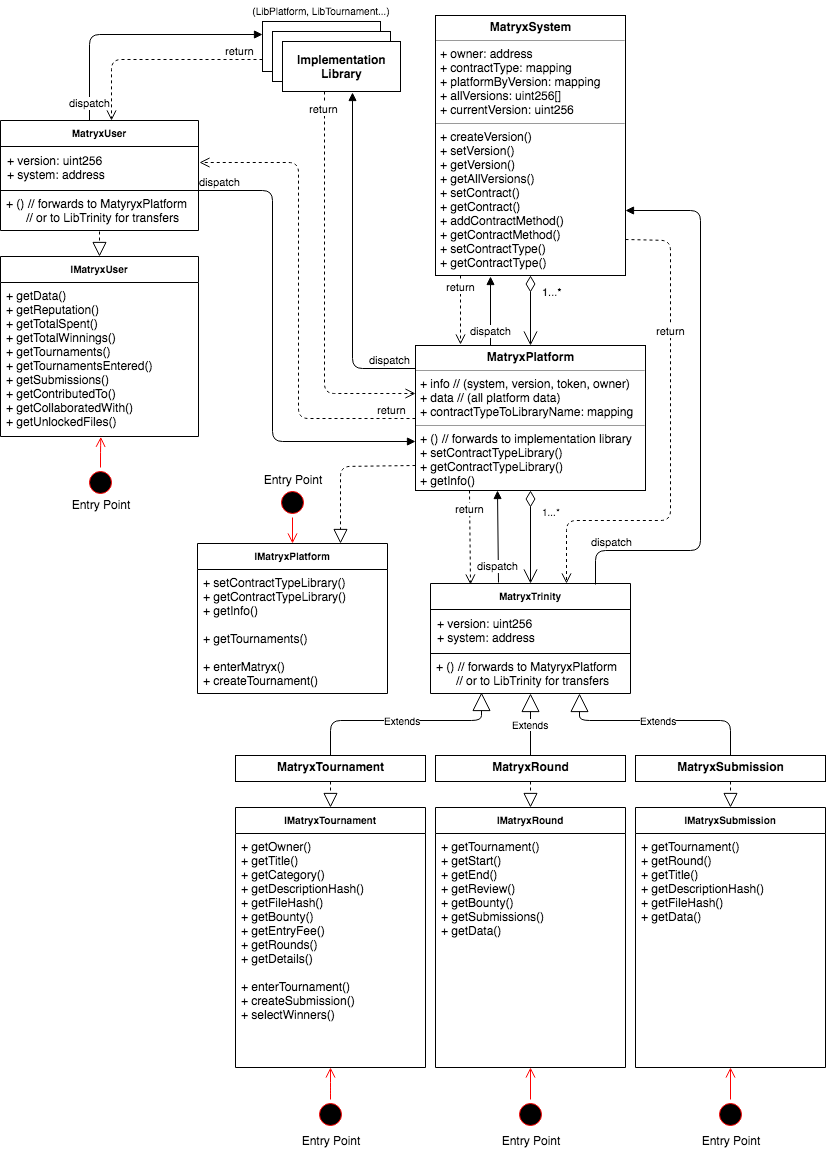
\includegraphics[scale = .5]{../Figures/architecture.png}
\end{figure*}

\end{document}